\section{Introducción}
Existen diversas formas de calcular la TDF, una de ellas es usando la Transformada Rápida de Fourier (Fast Fourier Transform, FFT). Esta produce la misma salida que la TDF pero en un tiempo significativamente menor.
\\La principal diferencia entre la TDF y la FFT es el rendimiento (tiempo de ejecución) que tiene cada uno de los algoritmos. Siendo la FFT miles de veces más veloz que la TDF, por lo cual, es común que en el tratamiento de señales digitales el algoritmos usado por defecto para cualquier tipo de análisis sea la FFT.\\ La complejidad de la TDF es de: $O(N^2)$ mientras que el de la FFT es: $O(Nlog(N))$, esto hace referencia al número de operaciones que necesita cada algoritmo.\\ La FFT trabaja de forma que descompone una señal en el dominio del tiempo de N puntos a N señales en el dominio del tiempo de un solo punto. Posteriormente calcula el espectro en frecuencia de las N señales y finalmente estos espectros en frecuencia son sintetizados dentro de uno solo obteniendo así la salida. En la figura 1 se muestra un ejemplo de la descomposición de una señal:
\begin{figure}[H]
	\centering
	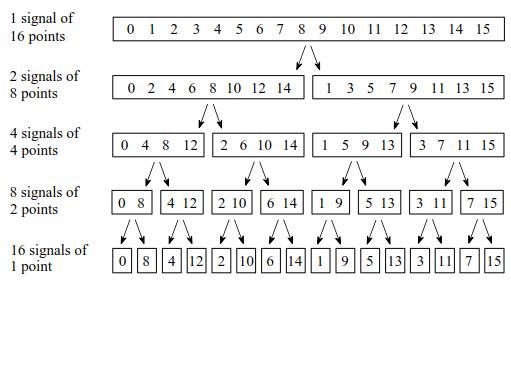
\includegraphics[scale=.8]{img/descomposicion.png}
	\caption{Descomposición de una señal de 16 puntos en 16 señales de 1 punto}
	\label{fig:prebSsDa2}		
\end{figure}
El número de fases de esta descomposición esta dado por $log_{2}(N)$. Posterior a esta descomposición, es necesario realizar un reordenamiento de las muestras, esto es logrado mediante la inversión de bits. El cual se puede observar en la siguiente figura:
\begin{figure}[H]
	\centering
	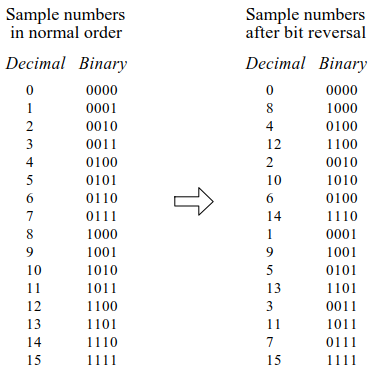
\includegraphics[scale=.8]{img/bit.png}
	\caption{Inversión de Bits}
	\label{fig:prebSsDa}		
\end{figure}
Después del reordenamiento es necesario encontrar el espectro en frecuencia de cada uno de los puntos, y después realizar la síntesis de los mismos fase por fase, al final se obtiene el resultado de la FFT.\\ Para esto se usa la siguiente operación, la cual es conocida coloquialmente como mariposa.
\begin{figure}[H]
	\centering
	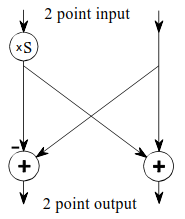
\includegraphics[scale=.82]{img/mariposa.png}
	\caption{Mariposa de la FFT}
	\label{fig:prebsDa}		
\end{figure}
En la Figura 4 se expone un diagrama completo sobre como funciona la FFT usando todas las descripciones antes mencionadas:
\begin{figure}[H]
	\centering
	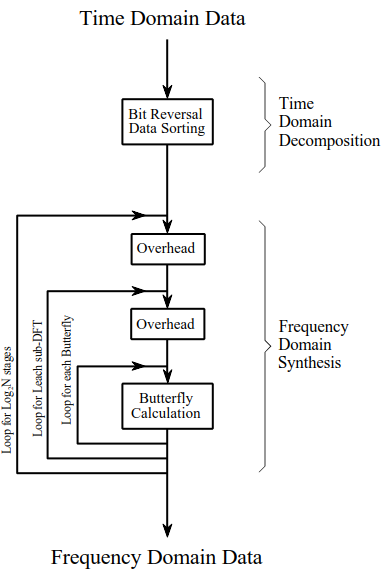
\includegraphics[scale=.7]{img/fft.png}
	\caption{Diagrama completo funcionamiento FFT}
	\label{fig:prebssDa}		
\end{figure}